\documentclass[aps,prb,onecolumn,notitlepage,showpacs,floatfix,superscriptaddress]{revtex4-1}
\usepackage{dcolumn}
\usepackage{tabularx}
\usepackage{bm}
\usepackage{soul}
\usepackage{amsmath,amssymb,graphicx}
\usepackage[colorlinks=true,citecolor=blue,urlcolor=blue,linkcolor=blue]{hyperref}
\usepackage{environ}

\NewEnviron{eqnsplit}{%
\begin{equation}
\begin{split}
  \BODY
\end{split}
\end{equation}
}

\newcommand{\mrm}[1]{\mathrm{#1}}
\newcommand{\ang}{\mathrm{\AA}}

\bibliographystyle{apsrev4-1}

%%%%%%%%%%%%%%%%%%%%%%%%%%%%%%%%%%%%%%%%%%%%%%%%
\begin{document}

\title{Weak Localization}

\author{Avinash Rustagi}
\email{arustag@ncsu.edu}
\affiliation{Department of Physics, North Carolina State University, Raleigh, NC 27695}
%
\date{\today}
%%%%%%%%%%%%%%%%%%%%%%%%%%%%%%%%%%%%%%%%%%%%%%%%

\maketitle
%
The variation of resistivity with temperature captures the temperature dependence of scattering mechanisms which dominate at different temperature regimes. For instance, the high temperature limit is resistivity is governed by phonon scattering $\rho \propto T$. At low temperatures, phonon modes are not occupied thus we can freeze the lattice degree of freedom, where impurity scattering is the dominant mechanism for resistivity $\rho = \text{Constant}$. The intermediate temperature regime is particularly interesting $T\approx T_D$ ($T_D$-Debye Temperature) where the Bloch Gruniessen power law shows up in resistivity temperature dependence $\rho \propto T^5$. This is due to phonon scattering restricted to small angles where $T^3$ behavior arises from the phonons and an additional $T^2$ comes about from phase space restrictions to scattering by small angles. 

Dolan and Osheroff observed a logarithmic decrease in resistivity with increase in temperature in two-dimensional PdAu thin films. This is now understood to have arisen from \textbf{Weak Localization}.
\begin{figure}[hbtp]
\centering
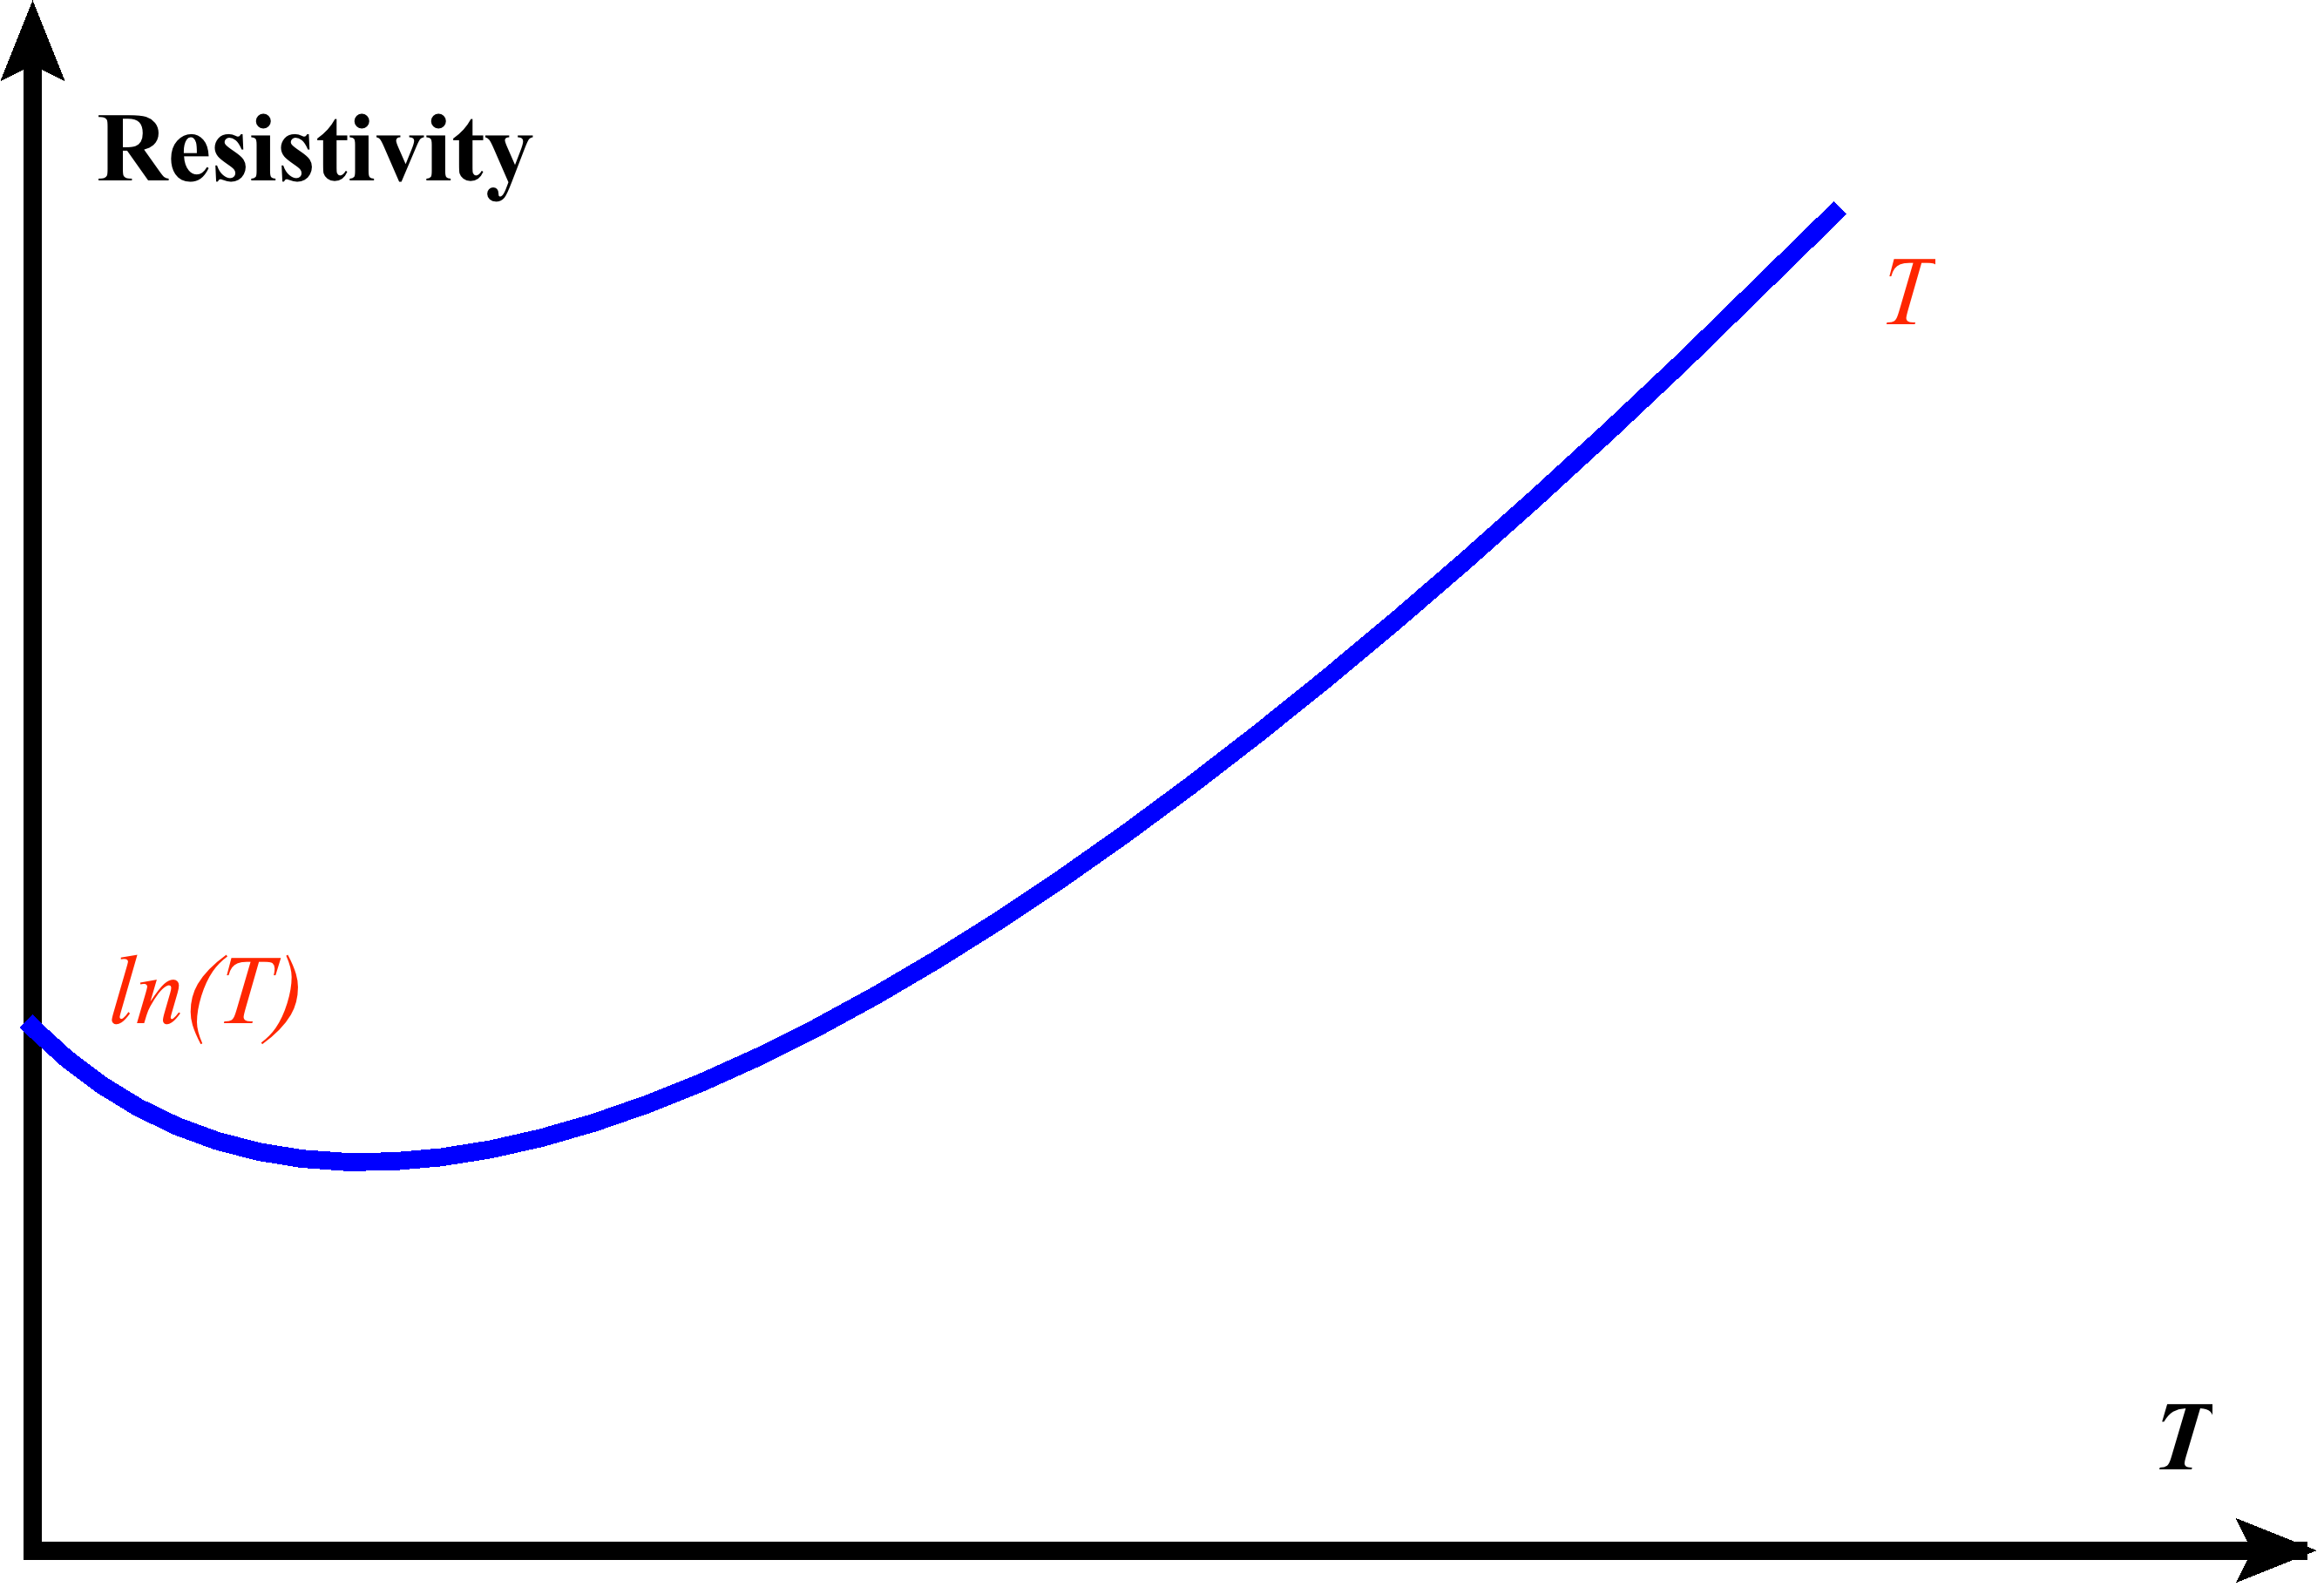
\includegraphics[scale=0.1]{Resistivity.png}
\caption{Resistivity vs Temperature}
\end{figure}

The concept of weak localization can be understood by considering the probability for an electron to return to its starting point after multiple scattering by impurities. The probability as we know is the square of the sum of all amplitudes corresponding to all possible paths. For returning to origin, say there exists a path 1 which has an amplitude $A_1$. There also exists a time-reversed path 2 which brings the electron back to its origin with amplitude $A_2$. If the system is time-reversal invariant, then the amplitudes of path 1 and 2 are equal $A_1=A_2=A$. Thus the probability of an electron returning to its starting position is
\begin{equation}
P_\mathrm{Origin} = \vert A_1 +A_2 \vert^2 = 4 \vert A \vert^2
\end{equation} 
Thus the probability increases 4-fold compared to the classical situation where the individual probabilities are added giving $\vert A_1 \vert^2+\vert A_2 \vert^2=2\vert A \vert^2$. The difference is due to constructive interference between the two paths. This is the basic idea behind weak localization.
\begin{figure}[hbtp]
\centering
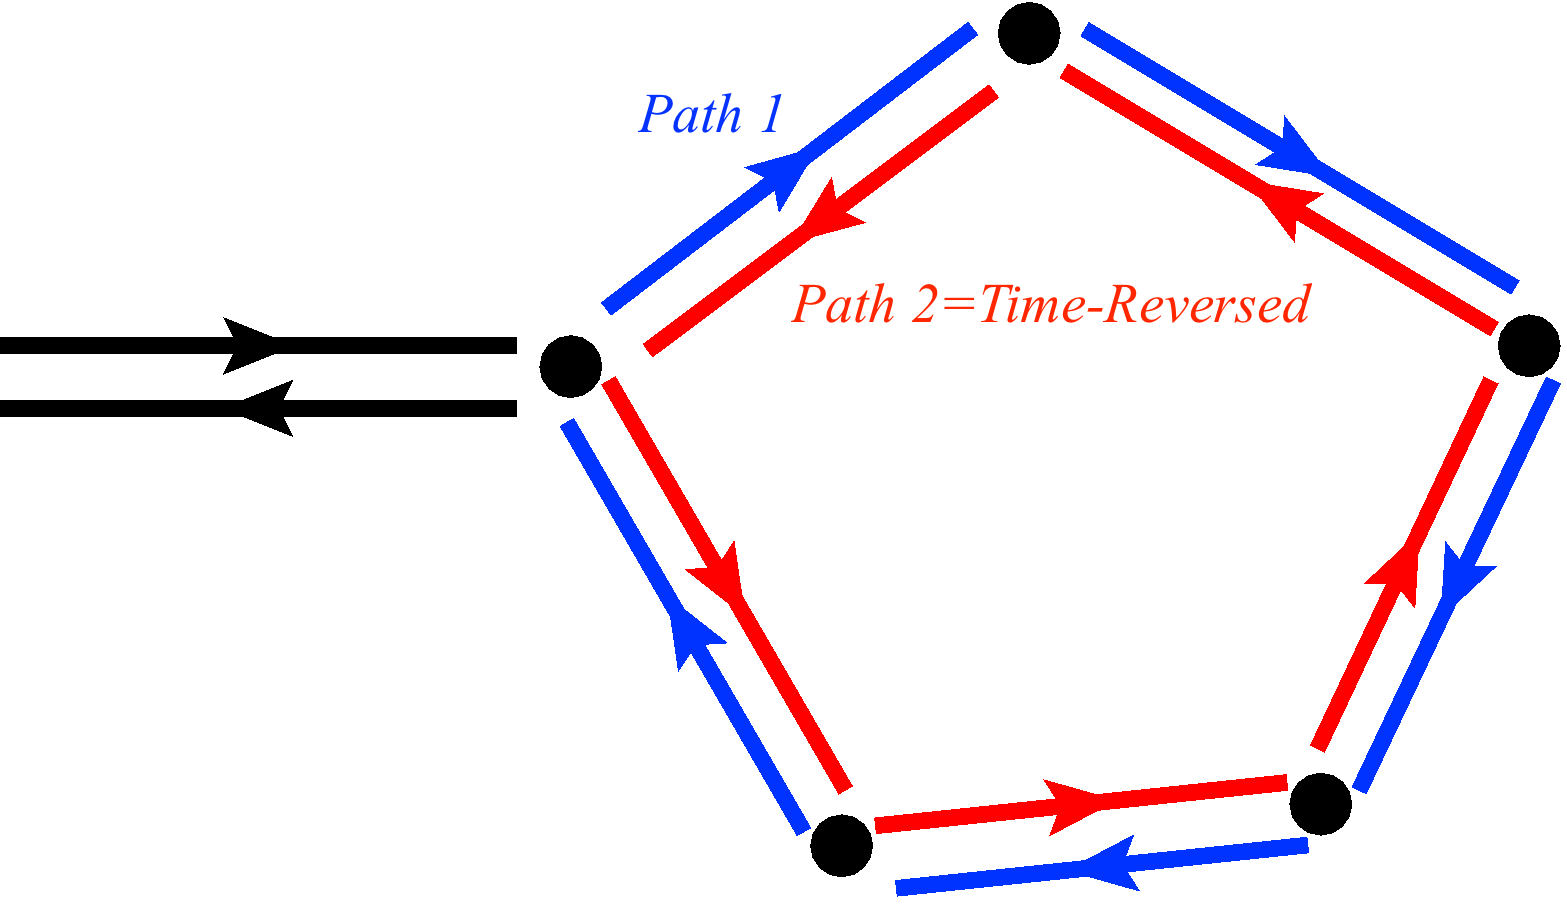
\includegraphics[scale=0.2]{TR_Paths.png}
\caption{Time-Reversed Path pairs contributing to backscattering i.e. return to origin.}
\end{figure}

\section{Diffusion Equation}
Let us consider the case of random walk in 1D.
\begin{itemize}
\item $l$ - step length of walker
\item $\tau$ - time for a single step
\item $p$ - probability of step to the right
\item $q=1-p$ - probability of step to the left
\item $P_N(m)$ - probability to find the walker at position $=ml$ at time $=N\tau$
\end{itemize}
We can simply construct an equation for the probability $P_N(m)$. 
\begin{equation}
P_{N+1}(m)=p P_N(m-1) +q P_N(m+1)
\end{equation}
For a non-biased walker, we can set $p=q=0.5$ which means the step to the right and left are equally likely.
\begin{equation}
P_{N+1}(m)=\dfrac{1}{2} P_N(m-1) + \dfrac{1}{2} P_N(m+1)
\end{equation}
Thus
\begin{equation}
P_{N+1}(m) - P_N(m)=\dfrac{1}{2} \left[ P_N(m-1) +  P_N(m+1) - 2P_N(m) \right]
\end{equation}
We can then use the definition of derivatives in finite-difference scheme and take the continuum limit
\begin{equation}
\begin{split}
\tau &\dfrac{\partial P}{\partial t} = \dfrac{1}{2} l^2 \dfrac{\partial^2 P}{\partial x^2}\\
&\dfrac{\partial P}{\partial t} =  D \dfrac{\partial^2 P}{\partial x^2}
\end{split}
\end{equation}
which is the Diffusion Equation with Diffusion Coefficient $D=l^2/2\tau$. The solution to this equation subject to the initial condition $P(x,t=0)=\delta(x)$ and boundary conditions $P(x=\pm\infty,t)=0$ is
\begin{equation}
P(x,t)=\dfrac{1}{\sqrt{2\pi \sigma^2}} \exp\left( -\dfrac{x^2}{2\sigma^2}\right)
\end{equation}
where $\sigma^2=2Dt$. The Diffusion Equation and its solution can be generalized to a d-dimensional space ($r^2=\sum_{i=1}^d x_i^2$)
\begin{equation}
\begin{split}
&\dfrac{\partial P}{\partial t} =  D \nabla^2 P \\
& P({\bm r},t)= \dfrac{1}{(2\pi \sigma^2)^{d/2}} \exp\left( -\dfrac{r^2}{2\sigma^2}\right)
\end{split}
\end{equation}

\section{Conductivity}
The probability density of returning to the origin ${\bm r}=0$
\begin{equation}
\begin{split}
& P({\bm r}=0,t)= \dfrac{1}{(4\pi Dt)^{d/2}} 
\end{split}
\end{equation}
An electron can be viewed as a wavepacket with linear extension given by Fermi wavelength $\lambda_F=1/k_F$. In a d-dimensional space this electron will sweep out a volume $\lambda_F^{d-1} v_F dt$ in the time interval $[t,t+dt]$. Thus interference is possible if the electron comes back to this volume about the origin. Also note that the electron coming back will cause a drop in conductivity (increase in resistivity). Therefore the change in conductivity is expressed as
\begin{equation}
\begin{split}
\dfrac{\delta \sigma}{\sigma_0} \approx - \int_{\tau}^{\tau_{\phi}} \dfrac{1}{(4\pi Dt)^{d/2}} \lambda_F^{d-1} v_F dt
\end{split}
\end{equation}
where $\tau$ is the scattering relaxation time, $\tau_{\phi}$ is the phase relaxation time. The integral can be evaluated in $d=1,2,3$ and 
\[ \dfrac{\delta \sigma}{\sigma_0} =\begin{cases} 
      -c_3 \dfrac{\lambda_F^2}{l^2} \left(1-\dfrac{\tau}{\tau_\phi} \right) & d=3 \\
      -c_2 \dfrac{\lambda_F}{l}\log\left(\dfrac{\tau_\phi}{\tau} \right)  & d=2 \\
      -c_1 \left( \sqrt{\dfrac{\tau_\phi}{\tau}}-1\right) & d=1 
   \end{cases}
\]
where mean free path $l=v_F \tau$. \\

\subsection{Weak Localization in 2D}
For Weak Localization $\tau_\phi > \tau$, since we want multiple scatterings to takes place and bring the electron to its origin however phase coherence should be maintained for interference. The phase relaxation rate is proportion to temperature $\tau_\phi^{-1} \propto T^\alpha$ since phase coherence is lost when scattering between electrons or with phonons takes place. This means that phase relaxation time decreases with increase in temperature which implies $\log(\tau_\phi / \tau)$ decreases. Thus the change in conductivity become less negative with increase in temperature which is the same as increase in conductivity.

\end{document}